\documentclass[12pt]{report}
\usepackage[thinc]{esdiff} % for typesettign derivatives
\usepackage{amsthm} % provides an enhanced version of LaTex's \newtheorem command
\usepackage{mdframed} % framed environments that can split at page boundaries
\usepackage{enumitem} % bulletin points or other means of listing things
\usepackage{amssymb} % for AMS symbols
\usepackage{amsmath} % so as to use align
\usepackage{latexsym} % so as to use symbols like \leadsto
\usepackage{mathrsfs} % for using mathscr for char like operators
\usepackage{commath} % for using norm symbol
\usepackage{authblk} % for writing affiliations
\usepackage{graphicx} % for importing images
\graphicspath{{./images/}} % for the path to images, also always put label behind captions
\usepackage{textcomp} % for using degree symbol
\usepackage{hyperref} % for clickable link in the pdf & customizable reference text
\usepackage[all]{hypcap} % for clickable link to images instead of caption
\usepackage[margin=1in]{geometry} % default is 1.5in
% \usepackage[left=0.4in, right=0.4in, top=0.8in, bottom=0.8in]{geometry}
\usepackage[title]{appendix} % for attaching appendix
\allowdisplaybreaks % allow page breaking in display maths, like align
% allow for more advanced table layout
\usepackage{booktabs}
\usepackage{multirow}
\usepackage{siunitx}
% for adjusting caption settings
\usepackage{caption}
\captionsetup[table]{skip=10pt}

\theoremstyle{definition}
\mdfdefinestyle{defEnv}{%
  hidealllines=false,
  nobreak=true,
  innertopmargin=-1ex,
}

% The following is for writing block of code
\usepackage{listings}
\usepackage{color}

\definecolor{dkgreen}{rgb}{0,0.6,0}
\definecolor{gray}{rgb}{0.5,0.5,0.5}
\definecolor{mauve}{rgb}{0.58,0,0.82}

\setlength{\parindent}{0pt}
\setlength{\fboxrule}{2pt}

% Use the following to change code language and related settings
\lstset{frame=tb,
  language=Python,
  aboveskip=3mm,
  belowskip=3mm,
  showstringspaces=false,
  columns=flexible,
  basicstyle={\small\ttfamily},
  numbers=none,
  numberstyle=\tiny\color{gray},
  keywordstyle=\color{blue},
  commentstyle=\color{dkgreen},
  stringstyle=\color{mauve},
  breaklines=true,
  breakatwhitespace=true,
  tabsize=3
}

\pagestyle{headings}
\author{Lectured by Alex Geringer-Sameth}
\title{Probability and Statistics for JMC}
\affil{Typed by Aris Zhu Yi Qing}
\begin{document}
\maketitle
\tableofcontents

\chapter{Review of Elementary Set Theory}

\noindent\fbox{%
    \parbox{\textwidth}{%
        \begin{align*}
            \Omega & \qquad\text{universal set} \\
            \medskip
            \emptyset & \qquad\text{empty set} \\
            \medskip
            A\subseteq\Omega & \qquad\text{subset of $\Omega$} \\
            \medskip
            \overline{A} & \qquad\text{Complement of $A$} \\
            \medskip
            |A| & \qquad\text{cardinality of $A$} \\
            \medskip
            A\cup B & \qquad\text{union ($A$ or $B$)} \\
            \medskip
            A\cap B & \qquad\text{intersection($A$ and $B$)} \\
            \medskip
            A=B & \qquad\text{both sets have exactly the same elements} \\
            \medskip
            A\backslash B & \qquad\text{set difference (elements in $A$ that are
            not in $B$)} \\
            \medskip
            \left\{\omega\right\} & \qquad\text{a singleton with only the
            element $\omega$ in the set} \\
            \medskip
            A\times B & \qquad\left\{(a,b)|a\in A, b\in B\right\}
        \end{align*}  
    }%
}

\chapter{Visual and Numerical Summaries}

\section{Visualization}

\begin{figure}
  	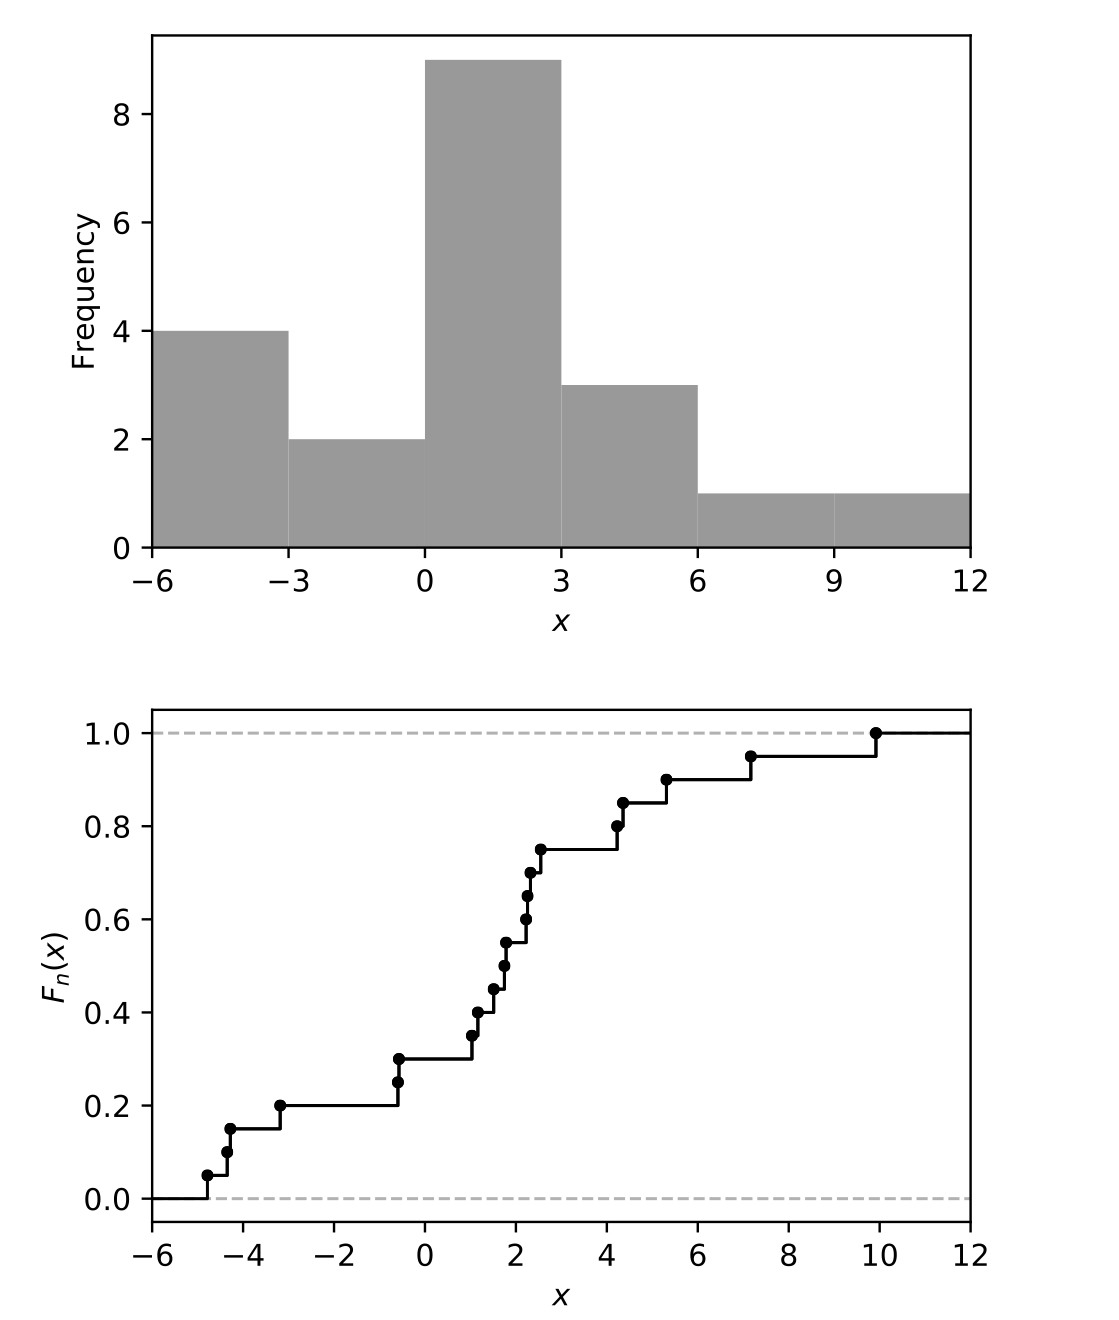
\includegraphics[scale=0.4]{./images/histogram_empirical_CDF.jpeg}
  	\centering
    \caption{The first diagram is the histogram, and the second diagram is the
    empirical cdf with the same set of data}\label{hist_cdf}
\end{figure}


\newmdtheoremenv[style=defEnv]{theorem}{Definition}
\begin{theorem}
The \textbf{\emph{histogram}} allows us to visualize how a sample of data
is distributed, say the observed values are $\left\{x_1,\ldots,x_2\right\}$.
The first step is deciding on a set of \textbf{\emph{bins}} that divide the
range of $x$ into a series of intervals.
A histogram then shows the \textbf{\emph{frequency}} for each bin.
\end{theorem}
\paragraph{\underline{Comments}}
Often the histogram's $y$-axis is normalized in some way.
\begin{itemize}
    \item 
        Instead of showing frequency, the height of the histogram can show
        \textbf{\emph{relative frequency}}, the fraction of the data set contained within the
        bin. 
        In this case, $1=\sum_{\text{bins }i} y_i$, where $y_i$ is the relative
        frequency at bin $i$.
    \item 
        The histogram could also show the \textbf{\emph{density}}, the relative
        frequency divided by the bin width.
        In this case, $1=\sum_{\text{bins }i} \rho_i\Delta x_i$, where $\rho_i$
        is the density for bin $i$ and $\Delta x_i$ is the width of bin $i$.
\end{itemize} 

\newmdtheoremenv[style=defEnv]{empirical CDF}[theorem]{Definition}
\begin{empirical CDF}
    The \textbf{\emph{empirical cumulative distribution function}} of a sample of
    real values $\left\{x_1,\ldots,x_n\right\}$ is
    \[
        F_n(x)=\frac{1}{n}\sum_{i=1}^{n} I(x_i\le x),
    \]
    where $I(x_i\le x)$ is an \textbf{\emph{indicator function}}, i.e.\ the
    value is 1 when $x_i\le x$ and 0 when $x_i>x$.
\end{empirical CDF}

\section{Summary Statistics}

\subsection{Measures of Location}

\noindent\fbox{%
    \parbox{\textwidth}{%
        \begin{align*}
            \text{arithmetic mean} & \qquad \overline{x}=\frac{1}{n}\sum_{i=1}^{n} x_i \\
            \text{geometric mean} & \qquad x_G={\left(\prod_{i=1}^{n}
            x_i\right)}^{\frac{1}{n}} \\
            \text{harmonic mean} &  \qquad\frac{1}{x_H}=\frac{1}{n}\sum_{i=1}^{n}
            \frac{1}{x_i} \\
            \text{$i^{\text{th}}$ order statistic} & \qquad x_{(i)}= \text{the
            $i^{\text{th}}$ smallest value of the sample} \\
            \text{median} &\qquad x_{\left(\frac{n+1}{2}\right)} \\
            \text{mode} & \qquad \text{$x_i$ which occurs most
            frequently in the sample}
        \end{align*} 
    }%
}
\paragraph{\underline{Comments}}
\begin{itemize}
        \item For positive data $\left\{x_1,\ldots,x_n\right\}$,
            \[
                \text{arithmetic mean}\ge\text{geometric mean}\ge\text{harmonic
                mean}.
            \]
        \item Arithmetic mean and geometric mean are related in the following
            way:
            \[
                \overline{x} = \frac{1}{n}\sum_{i=1}^{n} x_i =
                \frac{1}{n}\sum_{i=1}^{n} \ln{y_i} =
                \frac{1}{n}\ln{\prod_{i=1}^{n} y_i} =
                \ln{{\left(\prod_{i=1}^{n} y_i\right)}^{\frac{1}{n}}} =
                \ln{x_G},
            \]
            where $x_i = \ln{y_i}$.
        \item
            For $x_{(i)}$, when $i$ is not an integer, we define
            $\alpha\in(0,1)$ s.t. $\alpha=i-\lfloor i\rfloor $, and
            \[
                x_{(i)}=(1-\alpha)x_{(\lfloor i\rfloor)} 
                + \alpha x_{(\lceil i\rceil )}.
            \]
\end{itemize} 

\subsection{Measures of Dispersion}

\noindent\fbox{%
    \parbox{\textwidth}{%
        \begin{align*}
            \text{mean square/sample variance} & \qquad
            s^{2}=\frac{1}{n}\sum_{i=1}^{n} {(x_i-\overline{x})}^{2} \\
            \text{root mean square/sample standard deviation} & \qquad
            s = \sqrt{s^{2}} \\
            \text{range} & \qquad x_{(n)}-x_{(1)} \\
            \text{first quartile} & \qquad x_{\left(\frac{1}{4}(n+1)\right)} \\
            \text{third quartile} & \qquad x_{\left(\frac{3}{4}(n+1)\right)} \\
            \text{interquartile range} & \qquad 
            x_{\left(\frac{1}{4}(n+1)\right)} - x_{\left(\frac{3}{4}(n+1)\right)}
        \end{align*} 
    }%
}
\paragraph{Comments}
\begin{itemize}
        \item sample variance's different expression:
            \[
                s^{2} = \frac{1}{n}\sum_{i=1}^{n} {(x_i-\overline{x})}^{2}
                = \left(\frac{1}{n}\sum_{i=1}^{n} x_i^2\right)
                - {\left(\frac{1}{n}\sum_{i=1}^{n} x_i\right)}^{2}
                = \overline{x^{2}}-\overline{x}^{2}.
            \]
        \item Robustness, shown in table~\ref{robustness}
            \begin{table}[h]
                \centering
                \caption{Robustness of different location and dispersion statistic}
                \label{robustness}
                \begin{tabular}{l||c|c|c}
                    & Least Robust & More Robust & Most Robust \\
                    \hline\hline
                    Location & $\frac{x_{(1)}+x_{(n)}}{2}$ & $\overline{x}$ &
                    $x_{\left(\frac{n+1}{2}\right)}$ \\
                    \hline
                    Dispersion & $x_{(n)}-x_{(1)}$ & $s$ &
                    $x_{\left(\frac{3}{4}(n+1)\right)}-x_{\left(\frac{1}{4}(n+1)\right)}$
                \end{tabular} 
            \end{table} 
\end{itemize} 

\subsection{Covariance, Correlation, and Skewness}

\noindent\fbox{%
    \parbox{\textwidth}{%
        \begin{align*}
            \text{covariance} & \qquad s_{xy}=\frac{1}{n}\sum_{i=1}^{n}
            (x_i-\overline{x})(y_i-\overline{y}) \\
            \text{correlation} & \qquad r_{xy}=\frac{s_{xy}}{s_xs_y} \\
            \text{skewness} & \qquad \frac{1}{n}\sum_{i=1}^{n} 
            {\left(\frac{x_i-\overline{x}}{s}\right)}^{3}
        \end{align*} 
    }%
}
\paragraph{Comments}
\begin{itemize}
        \item covariance's different expression:
            \[
                s_{xy}=\frac{1}{n}\sum_{i=1}^{n}
                (x_i-\overline{x})(y_i-\overline{y})
                = \frac{1}{n}\sum_{i=1}^{n} x_iy_i+
                \frac{1}{n}\sum_{i=1}^{n} -x_i \overline{y}
                -\overline{x}y_i+\overline{x}\overline{y}
                = \frac{\sum_{i=1}^{n} x_iy_i}{n}
                -\overline{x}\,\overline{y}.
            \]
            In the random variable's context, it is
            \[
                \text{Cov}(X,Y)=E(XY)-E(X)E(Y).
            \]
        \item Correlation gives a \textbf{scale-invariant}
            measurement of relatedness between $x$ and $y$, since
            \[
                |r_{xy}|\le 1.
            \]
        \item A sample is \textbf{positively (negatively)} or
            \textbf{right (left) skewed} if the upper tail of the histogram of
            the sample is longer (shorter) than the lower tail.
\end{itemize} 

\subsection{Box-and-whisker plot}

The diagram is based on the five-point summary (use Figure~\ref{box-plot} as
reference):
\begin{itemize}
    \item Median -- middle line in the box.
    \item 3\textsuperscript{rd} and 1\textsuperscript{st} Quartiles -- top and
        bottom of the box.
    \item ``Whiskers'' -- extend out as dashed lines from the box to max/min
        values, which are the two short horizontal lines.
    \item Any outliers, i.e.\ extreme points beyond the whiskers, are plotted
        individually as dots.
\end{itemize} 
\begin{figure}[h]
  	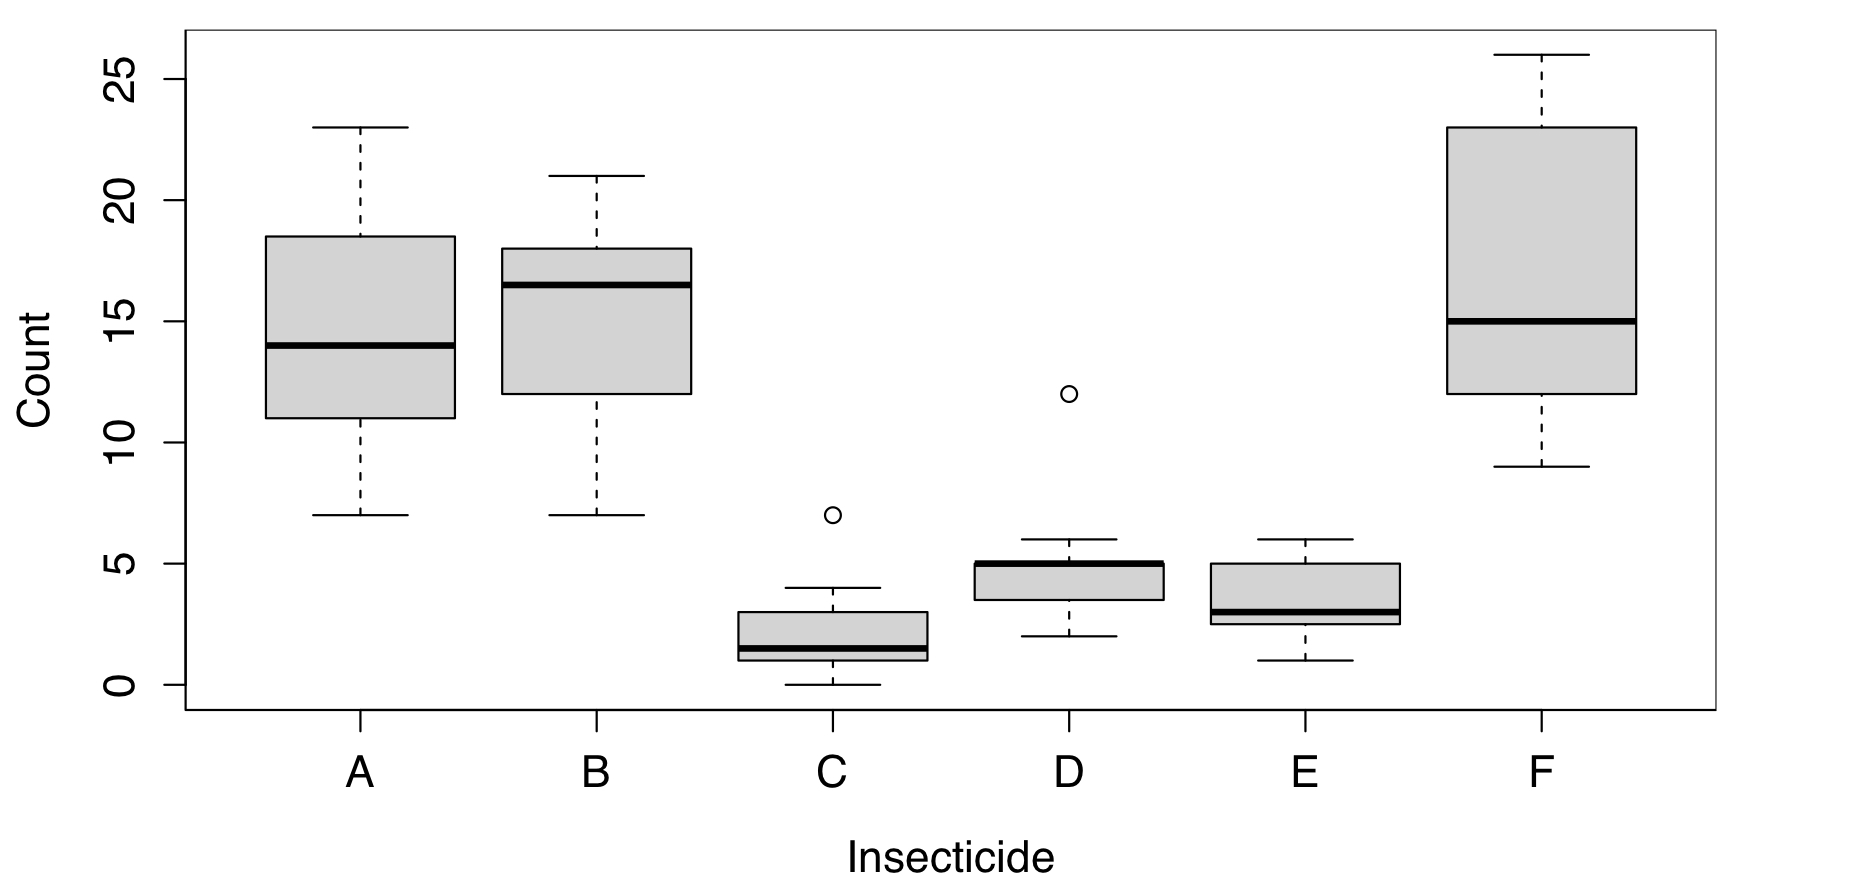
\includegraphics[scale=0.18]{./images/box-and-whisker.jpeg}
  	\centering
  	\caption{the counts of insects found in agricultural experimental units
    treated with six different insecticides A-F}\label{box-plot}
\end{figure}

\chapter{Probability}

\section{Formal Definition of Probability}

\subsection{$\sigma$-algebra}

\newmdtheoremenv[style=defEnv]{sigma algebra}[theorem]{Definition}
\begin{sigma algebra}\label{sigma-algebra}
    $\mathcal{F}$, a collection of subsets of a set $S$,
    is called a \textbf{\emph{$\sigma$-algebra}} associated with
    $S$ if:
    \begin{enumerate}[label = (\alph*)]
        \item $S\in\mathcal{F}$,
        \item $\mathcal{F}$ is closed under complements w.r.t. $S$:
            \[
                E\in\mathcal{F} \Longrightarrow \overline{E}\in\mathcal{F},
            \]
        \item $\mathcal{F}$ is closed under countable unions:
            \[
                E_1,E_2,\ldots\in\mathcal{F}\Longrightarrow
                \bigcup_{i=1}^{\infty}E_i\in\mathcal{F}.
            \]
    \end{enumerate} 
\end{sigma algebra}

\paragraph{Comments}
Definition~\ref{sigma-algebra} implies two facts.
\begin{enumerate}
    \item $\mathcal{F}$ must contain the empty set $\emptyset$.
        \begin{proof}
            Since $S\in\mathcal{F}$, we have
            $\overline{S}=\emptyset\in\mathcal{F}$.
        \end{proof} 
    \item $\mathcal{F}$ must be closed under countable intersections.
        \begin{proof}
            Let $E_1,E_2,\ldots\in\mathcal{F}$. We can then imply the following:
            \[
                \overline{E_1},\overline{E_2},\ldots\in\mathcal{F}
                \Rightarrow \bigcup_i \overline{E_i}\in\mathcal{F}
                \Rightarrow \overline{\bigcup_i \overline{E_i}}\in\mathcal{F}
                \xrightarrow{\text{De Morgan's Law}}\bigcap_iE_i\in\mathcal{F}.
            \]
        \end{proof} 
\end{enumerate} 
In short, we can take unions, intersections, and complements of members of
$\mathcal{F}$ in any combination and the result will always be a member of
$\mathcal{F}$.

\subsection{Probability Measure}

\newmdtheoremenv[style=defEnv]{probability measure and space}[theorem]
{(Kolmogorov's axioms of probability) Definition}
\begin{probability measure and space}
    A \textbf{\emph{probability measure}} $P$ is a function
    $P:\mathcal{F}\mapsto\mathbb{R}$ satisfying
    \begin{enumerate}[label = (\alph*)]
        \item $P(E)\ge 0 \;\forall E\in\mathcal{F}$,
        \item $P(S)=1$,
        \item If $E_1,E_2,\ldots\in\mathcal{F}$ are disjoint (i.e.\ $E_i\cap
            E_j=\emptyset \;\forall i\neq j$) then
            \[
                P\left(\bigcup_{i=1}^{\infty}E_i\right)=
                \sum_{i=1}^{\infty} P(E_i).
            \]
    \end{enumerate} 
    The triplet $(S,\mathcal{F},P)$, consisting of a set $S$, a $\sigma$-algebra
    $\mathcal{F}$ of subsets of $S$, and a probability measure $P$, is called a
    \textbf{\emph{probability space}}.
\end{probability measure and space}

\paragraph{Comments}
\begin{itemize}
    \item The \textbf{\emph{sample space}} $(S)$ is the set of all possible
        outcomes of an experiment.
    \item The \textbf{\emph{event space}} $(\mathcal{F})$ is the set of possible
        events, where an \textbf{\emph{event}} $E$ is a subset of the sample
        space, $E\subseteq S$. An \textbf{\emph{elementary event}} is one that
        consist of a single element of $S$, i.e.\ a singleton.
    \item The probability measure $(P)$ has three important interpretations:
        \begin{enumerate}
            \item \textbf{classical}:
                Different outcomes in the sample space $S$ 
                are ``equally likely'',
            \item \textbf{frequentist}:
                the relative frequency of an event over many trials,
            \item \textbf{subjective}:
                a numerical measure of the degree of belief held by an individual.
        \end{enumerate} 
        \newtheorem{probability-interpretations}[theorem]{Example}
        \begin{probability-interpretations}
            ``A sensor can detect items within 10 cm of the sensor.
            The sensor is placed in a room together with an object, and
            the probability that the sensor makes a detection is 0.0001.''
            \begin{enumerate}
                \item \textbf{classical}:
                    The volume within 10 cm of the sensor divided by the volume
                    of the room is 0.0001.
                \item \textbf{frequentist}:
                    If we repeat the experiment a lot of times, then the
                    fraction of the experiments in which the sensor makes a
                    detection is 0.0001.
                \item \textbf{subjective}:
                    Someone's subjective degree of belief, measured on a
                    numerical scale from 0 to 1, that the sensor will detect is
                    0.0001.
            \end{enumerate} 
        \end{probability-interpretations}
    \item several results that can be derived from the probability measure
        axioms:
        \begin{itemize}
            \item $P(\emptyset)=0$.
            \item $P(E)\le 1$.
            \item $P(\overline{E})=1-P(E)$.
            \item $P(E\cup F)=P(E)+P(F)-P(E\cap F)$..
            \item $P(E\cap \overline{F})=P(E)-P(E\cap F)$.
            \item If $E\subset F$ then $P(E)\le P(F)$.
        \end{itemize} 
\end{itemize} 

\section{Conditional Probability}

\newmdtheoremenv[style=defEnv]{conditional probability}[theorem]{Definition}
\begin{conditional probability}
    If $P(F)>0$ then the \textbf{\emph{conditional probability}} of $E$ given
    $F$ is
    \[
        P(E|F)=\frac{P(E\cap F)}{P(F)}.
    \]
\end{conditional probability}
\paragraph{Comments}
\begin{itemize}
    \item Difference among the following forms:
        \begin{itemize}
            \item $P(E|F)$ -- \textbf{\emph{conditional probabilities}},
            \item $P(E\cap F)$ -- \textbf{\emph{joint probabilities}},
            \item $P(E)$ -- \textbf{\emph{marginal probabilities}}.
        \end{itemize} 
    \item several results derived from the conditional probability definition:
        \begin{itemize}
            \item $P(E|F)\ge 0$ for any event $E$.
            \item $P(F|F)=1$.
            \item If the events $E_1,E_1,\ldots$ are pairwise disjoint, then
                $P\left(\left(\bigcup_i E_i\right)|F\right)=\sum_{i} P(E_i|F)$.
        \end{itemize} 
    \item \underline{Warning}: In general, $P(E|F)\neq P(F|E)$.
\end{itemize} 

\newtheorem{conditional probability eg}[theorem]{Example}
\begin{conditional probability eg}
    A medical test for a disease $D$ has outcomes $+$ and $-$.
    The probabilities are
    \begin{table}[h]
        \centering
        \begin{tabular}{l||c|c|c}
            & $D$ & $\overline{D}$ & \\
            \hline\hline
            $+$ & 0.009 & 0.099 & 0.108 \\
            \hline
            $-$ & 0.001 & 0.891 & 0.892 \\
            \hline
                & 0.01 & 0.99 &
        \end{tabular} 
    \end{table} 

    By the definition of conditional probability, we have
    \[
        P(+|D)=90\%,\quad P(-|\overline{D})=90\%, \quad
        P(D|+)=\frac{0.009}{0.108}\approx 0.083.
    \]
    The first two probabilities show that the test is fairly accurate. Sick
    people yield a positive 90\% of the time and healthy people yield a negative
    90\% of the time.
\end{conditional probability eg}


\section{Independence}

\newmdtheoremenv[style=defEnv]{independence}[theorem]{Definition}
\begin{independence}
    Two events $E$ and $F$ are \textbf{\emph{independent}} iff
    \[
        P(E\cap F)=P(E)P(F).
    \]
\end{independence}
\paragraph{Comments}
\begin{itemize}
    \item Extension: The events $E_1,\ldots,E_k$ are independent if, for every
        subset of events of size $l\le k$, say indexed by
        $\left\{i_1,\ldots,i_l\right\}$,
        \[
            P\left(\bigcap_{j=1}^l E_{i_j}\right)=\prod_{j=1}^{l} P(E_{i_j}).
        \]
    \item Independence could be either assumed or verified via the definition.
    \item Disjoint events with positive probability are not independent.
    \item From the definition of conditional probability, we can deduce that
        $E$ and $F$ are independent iff $P(E|F)=P(E)$.
\end{itemize} 

\newmdtheoremenv[style=defEnv]{conditional independence}[theorem]{Definition}
\begin{conditional independence}
    For three events $E_1, E_2, F$, the pair of events $E_1$ and $E_2$ are
    said to be \textbf{\emph{conditionally independent given $F$}} iff
    \[
        P(E_1\cap E_2|F) = P(E_1|F)P(E_2|F).
    \]
    which could also be written as $E_1\bot E_2|F$.
\end{conditional independence}

\section{Bayes' Theorem}

\newmdtheoremenv[style=defEnv]{law of total probability}[theorem]{(The Law of
Total Probability) Theorem}
\begin{law of total probability}
    Let $E_1,E_2,\ldots$ be a partition of $S$,
    i.e.\ $E_i\cap E_j=\emptyset$ for $i\neq j$ and $\bigcup_i E_i=S$.
    Then, for any event $F\subseteq
    S$, we have
    \[
        P(F)=\sum_{i}P(F|E_i)P(E_i).
    \] 
\end{law of total probability}
\begin{proof}
    $P(F)=P(\bigcup_i F\cap E_i)=\sum_{i} P(F\cap E_i)=\sum_{i}P(F|E_i)P(E_i)$.
\end{proof} 

\newmdtheoremenv[style=defEnv]{bayes' theorem}[theorem]{(Bayes' Theorem) Theorem}
\begin{bayes' theorem}
    If $P(F)>0$ and let $E_1,E_2,\ldots$ be a partition on $S$ s.t. $P(E_i)>0
    \,\forall i$, we have
    \[
        P(E_i|F)=\frac{P(F|E_i)P(E_i)}{P(F)}
        = \frac{P(F|E_i)P(E_i)}{\sum_{j}P(F|E_j)P(E_j)},
    \]
    where $P(E_i|F)$ is called the \textbf{\emph{posterior}},
    $P(F|E_i)$ is called the \textbf{\emph{likelihood}},
    $P(E_i)$ is called the \textbf{\emph{prior}},
    and $P(F)$ is called the \textbf{\emph{evidence}}.
\end{bayes' theorem}
\begin{proof}
    Exercise! haha
\end{proof} 

\newtheorem{bayes' theorem eg}[theorem]{Example}
\begin{bayes' theorem eg}
    A new covid-19 test is claimed to correctly identify 95\% of people who are
    really covid-positive and 98\% of people who are really covid-negative.
    If only 1 in a 1000 of the population are infected, what is the probability
    that a randomly selected person who tests positive actually has the disease?

    \medskip
    Let $I$ = ``has a covid infection'' and $T$ = ``test is positive''.
    We are given $P(T|I)=0.95,P(\overline{T}|\overline{I})=0.98,P(I)=0.001$.
    We can thus derive that
    \[
        P(I|T)=\frac{P(T|I)P(I)}{P(T)}
        =\frac{P(T|I)P(I)}{P(T|I)P(I)+P(T|\overline{I})P(\overline{I})}
        = \frac{0.95\times 0.001}{0.95\times 0.001 + 0.02\times 0.999}
        = 0.045.
    \]
\end{bayes' theorem eg}

\chapter{Discrete Random Variables}

\section{Random Variables}

\newmdtheoremenv[style=defEnv]{random variable}[theorem]{Definition}
\begin{random variable}
    A \textbf{\emph{random variable}} is a (measurable) mapping
    \[
        X:S\mapsto\mathbb{R}
    \]
    with the property that 
    $\left\{s\in S:X(s)\le x\right\}\in\mathcal{F}\;\forall x\in\mathbb{R}$.
    This ensures that any set $B\subseteq\mathbb{R}$ corresponds to an event in
    the event space $\mathcal{F}$.
\end{random variable}

\newmdtheoremenv[style=defEnv]{range of X}[theorem]{Definition}
\begin{range of X}
    The image of $S$ under $X$ is called the \textbf{\emph{range}} of the random
    variable
    \[
        \mathbb{X}\equiv X(S)=\left\{X(s)|s\in S\right\}
        =\left\{x\in\mathbb{R}\,|\,\exists s\in S\text{ s.t. }X(s)=x\right\}.
    \]
    So $S$ contains all the possible outcomes of the experiment, 
    $\mathbb{X}$ contains all the possible outcomes of the random variable $X$.
\end{range of X}

\newmdtheoremenv[style=defEnv]{probability distribution}[theorem]{Definition}
\begin{probability distribution}
    The \textbf{\emph{probability distribution}} of $X$ is defined as
    \[
        P_X = P_X(X\in B\subseteq\mathbb{R}) 
        = P(\left\{s\in S:X(s)\in B\right\})
    \]
    which enables us to transfer the probability measure $P$ defined on $\mathcal{F}$
    to the real numbers in a natural way, and vice versa. For instance,
    \begin{align*}
        P_X(X=7) & = P(\left\{s\in S|X(s) = 7\right\}), \\
        P_X(a<X\le b) & = P(\left\{s\in S|a<X(s)\le b\right\}).
    \end{align*} 
\end{probability distribution}

\newtheorem{probability distribution application eg}[theorem]{Example}
\begin{probability distribution application eg}
    Consider counting the number of heads in a sequence of 3 coin tosses. The
    underlying sample space is
    \[
        S = \left\{TTT,TTH,THT,HTT,THH,HTH,HHT,HHH\right\}.
    \]
    Since we are only interested in the number of heads in each sequence,
    we define the random variable $X$ by
    \[
        X(s)=
        \begin{cases}
            0, & s=TTT,\\
            1, & s\in\left\{TTH,THT,HTT\right\}, \\
            2, & s\in\left\{HHT,HTH,THH\right\}, \\
            3, & s=HHH.
        \end{cases} 
    \]
    Thus, the probability of the number of heads $X$ is less than 2 is
    \begin{align*}
        P_X(X<2)
        & =P(\left\{s\in S:X(s)<2\right\}) \\
        & =P(\left\{TTT,TTH,THT,HTT\right\}) \\
        & =\frac{\left|\left\{TTT,TTH,THT,HTT\right\}\right|}{|S|} \\
        & =\frac{4}{8}= \frac{1}{2}.
    \end{align*} 
    On a side note, the above process uses the classical interpretation on the
    probability measure.
\end{probability distribution application eg}

\newmdtheoremenv[style=defEnv]{cdf}[theorem]{Definition}
\begin{cdf}
    The \textbf{\emph{Cumulative Distribution Function (CDF)}} of a random
    variable $X$ is the function $F_X:\mathbb{R}\mapsto[0,1]$, defined by
    \[
        F_X(x)=P_X(X\le x)=P(\left\{s\in S:X(s)\le x\right\}).
    \]
\end{cdf}
\paragraph{Comments}
\begin{itemize}
    \item Given a right-continuous function $F_X(x)$, check the following to
        verify if it is a valid CDF:
        \begin{enumerate}[label = (\roman*)]
            \item $0\le F_X(x)\le 1\;\forall x\in\mathbb{R}$,
            \item Monotonicity (non-decreasing):
                $\forall x_1,x_2\in\mathbb{R}, x_1<x_2\Rightarrow F_X(x_1)\le
                F_X(x_2)$.
            \item $F_X(-\infty)=0, F_X(\infty)=1$.
        \end{enumerate} 
    \item For finite intervals $(a,b]\subseteq\mathbb{R}$, it is easy to check
        that 
        \[
            P_X(a<X\le B)=F_X(b)-F_X(a).
        \]
    \item Usually we suppress the subscript of $P_X(\cdot)$ and just write
        $P(\cdot)$ for the probability measure for the random variable, unless
        there is any ambiguity.
\end{itemize} 

\section{Discrete Random Variables}

\newmdtheoremenv[style=defEnv]{discrete RV}[theorem]{Definition}
\begin{discrete RV}
    A random variable $X$ is \textbf{\emph{discrete}} if the range of $X$,
    $\mathbb{X}$, is countable, that is
    \[
        \mathbb{X}=\left\{x_1,x_2,\ldots,x_n\right\}\text{ (finite)}
        \quad\text{or}\quad 
        \mathbb{X}=\left\{x_1,x_2,\ldots\right\}\text{ (infinite)}.
    \]
\end{discrete RV}

\newmdtheoremenv[style=defEnv]{pmf}[theorem]{Definition}
\begin{pmf}
    For a discrete random variable $X$, we define the \textbf{\emph{Probability
    Mass Function (PMF)}} as\[
        p_X(x)=P_X(X=x),\quad x\in\mathbb{X}.
    \]
    For completeness, we also define
    \[
        p_X(x) = 0, \quad x\notin\mathbb{X}.
    \]
    so that $p_x$ is defined for all $x\in\mathbb{R}$.
\end{pmf}

\newmdtheoremenv[style=defEnv]{support}[theorem]{Definition}
\begin{support}
    The \textbf{\emph{support}} of a random variable $X$ is defined as
    \[
        \left\{x\in\mathbb{R}: p_X(x)>0\right\},
    \]
    which is \underline{almost always} the same as the range $\mathbb{X}$.
\end{support}

\subsubsection{Properties of $p_X$ and $F_X$}
\begin{itemize}
    \item $p_X(x_i)\ge 0$.
    \item $\sum_{x\in\mathbb{X}} p_X(x)=1$.
    \item $F_X(x)=P(X\le x)$, $x\in\mathbb{R}$.
    \item Let $X$ be a discrete random variable with range
        $\mathbb{X}=\left\{x_1,x_2,\ldots\right\}$, where $x_1<x_2<\ldots$.
        Then for any $x\in\mathbb{R}$, if $x<x_1$, $F_X(x)=0$; otherwise
        \[
            F_X(x)=\sum_{x_i\le x} p_X(x_i) \iff p_X(x_i)=F_X(x_i)-F_X(x_{i-1}),
                \quad i=2,3,\ldots,
        \]
        with $p_X(x_1)=F_X(x_1)$.
    \item $\lim_{x\rightarrow-\infty}F_X(x)=0$,
        $\lim_{x\rightarrow\infty}F_X(x)=1$.
    \item $F_X$ is continuous from the right on $\mathbb{R}$, i.e.\ for
        $x\in\mathbb{R}$, $\lim_{h\rightarrow 0^{+}}F_X(x+h)=F_X(x)$.
    \item $F_X$ is non-decreasing, i.e.\
        $a<b \Longrightarrow F_X(a)\le F_X(b)$.
    \item For $a<b$, $P(a<X\le b)=F_X(b)-F_X(a)$.
\end{itemize} 

\section{Functions of a Discrete Random Variable}

\newmdtheoremenv[style=defEnv]{pmf of g(X)}[theorem]{Definition}
\begin{pmf of g(X)}
    The PMF of $Y=g(X)$ is found by grouping all the values in the range of $x$
    that correspond to the same value of $Y$, i.e.\
    \[
        p_{Y}(y)=\sum_{x\in\mathbb{X}:g(x)=y} p_X(x).
    \]
\end{pmf of g(X)}

\section{Mean and Variance}

\newmdtheoremenv[style=defEnv]{mean}[theorem]{Definition}
\begin{mean}
    The \textbf{\emph{expected value}}, or \textbf{\emph{mean}} of a discrete
    random variable $X$ is defined to be 
    \[
        E_X(X)=\sum_{x\in\mathbb{X}} xp_X(x),
    \]
    which is often written as $E(X)$, $E[X]$, or $\mu_X$.
\end{mean}

\newmdtheoremenv[style=defEnv]{E(g(X))}[theorem]{Theorem}
\begin{E(g(X))}
    \[
        E(g(X))=\sum_{x\in\mathbb{X}} g(x)p_X(x).
    \]
\end{E(g(X))}
\begin{proof}
    Let $Y=g(X)$, then
    \begin{align*}
        E(Y) & = \sum_{y\in \mathbb{Y}} yp_Y(y) \\
             & = \sum_{y\in \mathbb{Y}} y \sum_{x\in\mathbb{X}:g(x)=y} p_X(x) \\
             & = \sum_{y\in \mathbb{Y}} \sum_{x\in\mathbb{X}:g(x)=y} g(x)p_X(x) \\
             & = \sum_{x\in\mathbb{X}} g(x)p_X(x).
    \end{align*} 
\end{proof} 

\newmdtheoremenv[style=defEnv]{linearity of expectation}[theorem]{Theorem}
\begin{linearity of expectation}
    Let $X$ be a random variable with $p_X$. Let $g$ and $h$ be real-valued
    functions, $g,h:\mathbb{R}\mapsto\mathbb{R}$, and let $a$ and $b$ be
    constants. Then
    \[
        E(ag(X)+bh(X)) = aE(g(X))+bE(h(X)).
    \]
\end{linearity of expectation}
\begin{proof}
    Exercise!
\end{proof} 

\newmdtheoremenv[style=defEnv]{variance}[theorem]{Definition}
\begin{variance}
    Let $X$ be a random variable. The \textbf{\emph{variance}} of $X$, denoted
    by $\sigma^{2}$ or $\sigma_X^{2}$ or $\text{Var}_X(X)$,
    is defined by
    \[
        \text{Var}_X(X)=E_X\left[{(X-E_X(X))}^{2}\right].
    \]
\end{variance}

\newmdtheoremenv[style=defEnv]{variance alternate form}[theorem]{Proposition}
\begin{variance alternate form}
    \[
        \text{Var}(X)=E(X^{2})-E(X)^{2}.  
    \]
\end{variance alternate form}
\begin{proof}
    \begin{align*}
        \text{LHS} & = E\left[X^{2}-2E(X)X+E(X)^{2}\right] \\
                   & = E(X^{2})-2E(X)E(X)+E(X)^{2} \\
                   & = \text{RHS}.
    \end{align*} 
\end{proof} 

\newmdtheoremenv[style=defEnv]{variance of sum of two RV}[theorem]{Proposition}
\begin{variance of sum of two RV}
    \[
        \text{Var}(aX\pm bY) = a^{2}\text{Var}(X)
        + b^{2}\text{Var}(Y) \pm 2ab\text{Cov}(X,Y).
    \]
\end{variance of sum of two RV}
\begin{proof}
    Exercise!
\end{proof} 

\newmdtheoremenv[style=defEnv]{standard deviation}[theorem]{Definition}
\begin{standard deviation}
    The \textbf{\emph{standard deviation}} of a random variable $X$, written
    $\text{sd}_X(X)$ or $\sigma_X$, is the square root of the variance,
    \[
        \sigma_X = \sqrt{\text{Var}_X(X)}.
    \]
\end{standard deviation}

\newmdtheoremenv[style=defEnv]{skewness of discrete RV}[theorem]{Definition}
\begin{skewness of discrete RV}
    The \textbf{\emph{skewness}} ($\gamma_1$) of a discrete random variable $X$
    is given by
    \[
        \gamma_1=\frac{E_X\left[{\left\{X-E_X(X)\right\}}^{3}\right]}{\sigma_X^{3}}.
    \]
\end{skewness of discrete RV}

\subsubsection{Sums of Random Variables}

Let $X_1,X_2,\ldots,X_n$ be $n$ random variables, perhaps with different
distributions and not necessarily independent. Let $S_n=\sum_{i=1}^{n} X_i$ be
the sum of those variables, and $\frac{S_n}{n}$ be their sample average. Both
$S_n$ and $\overline{S}=\frac{S_n}{n}$ are random variables themselves.

\bigskip
The mean of $S_n$ and $\frac{S_n}{n}$ are given by
\[
    E(S_n)=\sum_{i=1}^{n} E(X_i),\quad 
    E\left(\overline{S}\right)=\frac{\sum_{i=1}^{n} E(X_i)}{n}=\mu_X.
\]

If $X_1,X_2,\ldots,X_n$ are \textbf{independent}, we can calculate the variance
of $S_n$ and $\overline{S}=\frac{S_n}{n}$ as well:
\[
    \text{Var}(S_n)=\sum_{i=1}^{n} \text{Var}(X_i),\quad
    \text{Var}(\overline{S})=\frac{\sum_{i=1}^{n}
    \text{Var}(X_i)}{n^{2}}=\frac{\sigma_X^{2}}{n}.
\]

\section{Some important Discrete Random Variables}

\newmdtheoremenv[style=defEnv]{bernoulli distribution}[theorem]{Definition}
\begin{bernoulli distribution}
    We say $X$ follows a \textbf{\emph{Bernoulli Distribution}} if $X\sim 
    \text{Bernoulli}(p)$, where $0\le p\le 1$, and the pmf is given by
    \[
        p_X(x)=
        \begin{cases}
            p & x=1 \\
            1-p & x=0 \\
            0 & \text{otherwise}
        \end{cases} 
        = p^{x}{(1-p)}^{1-x}, \quad x\in\mathbb{X}=\left\{0,1\right\}.
    \]
\end{bernoulli distribution}

\newmdtheoremenv[style=defEnv]{bionomial distribution}[theorem]{Definition}
\begin{bionomial distribution}
    We say $X$ follows a \textbf{\emph{Binomial Distribution}} if $X\sim
    \text{Binomial}(n, p)$, where $0\le p \le 1$ and $n\in\mathbb{Z}^+$, 
    and the pmf is given by
    \[
        p_{X}(x)=\begin{pmatrix}
                n \\
                x
            \end{pmatrix} p^{x}{(1-p)}^{n-x}, \quad
            x\in\mathbb{X}=\left\{0,1,2,\ldots,n\right\}.
    \]
\end{bionomial distribution}

\newmdtheoremenv[style=defEnv]{geometric distribution}[theorem]{Definition}
\begin{geometric distribution}
    We say $X$ follows a \textbf{\emph{Geometric Distribution}} if $X\sim
    \text{Geometric}(p)$, where $0\le p\le 1$, and the pmf is given by
    \[
        p_{X}(x)=p{(1-p)}^{x-1}, \quad
        x\in\mathbb{X}=\left\{1,2,\ldots\right\}.
    \]
    Alternatively, let $Y=X-1$, then $Y\sim\text{Geometric}(p)$ with the pmf
    \[
        p_Y(y)=p{(1-p)}^{y}, \quad y\in\mathbb{N}=\left\{0,1,2,\ldots\right\}.
    \]
\end{geometric distribution}

\newmdtheoremenv[style=defEnv]{poisson distribution}[theorem]{Definition}
\begin{poisson distribution}
    We say $X$ follows a \textbf{\emph{Poisson Distribution}} if
    $X\sim\text{Poissons}(\lambda)$, where $\lambda>0$, and the pmf is given by
    \[
        p_X(x)=\frac{e^{-\lambda}\lambda^{x}}{x!}, \quad
        x\in\mathbb{X}=\left\{0,1,2,\ldots\right\}.
    \]
\end{poisson distribution}

\newmdtheoremenv[style=defEnv]{discrete uniform distribution}[theorem]{Definition}
\begin{discrete uniform distribution}
    We say $X$ follows a \textbf{\emph{Discrete Uniform Distribution}} if
    $X\sim$ Uniform(\{1, 2, \ldots, n\}), and the pmf is given by
    \[
        p_X(x)=\frac{1}{n}, \quad x\in\mathbb{X}=\left\{1,2,\ldots,n\right\}.
    \]
\end{discrete uniform distribution}

\begin{table}[h]
    \centering
    \caption{Means and Variances of different distributions}
    \label{mean_var_of_distributions}
    \def\arraystretch{2.3}
    \begin{tabular}{l||c|c|c}
        & Mean($\mu$) & Variance($\sigma^{2}$) & Skewness($\gamma_1$) \\
        \hline\hline
        Bernoulli & $p$ & $p(1-p)$ & N.A. \\
        Binomial & $np$ & $np(1-p)$ & $\dfrac{1-2p}{\sqrt{np(1-p)}}$ \\
        Geometric(original) & $\dfrac{1}{p}$ & $\dfrac{1-p}{p^{2}}$ &
        $\dfrac{2-p}{\sqrt{1-p}}$ \\
        Geometric(alternative) & $\dfrac{1-p}{p}$ & $\dfrac{1-p}{p^{2}}$
                               & $\dfrac{2-p}{\sqrt{1-p}}$ \\
        Poisson & $\lambda$ & $\lambda$ & $\dfrac{1}{\sqrt{\lambda}}$ \\
        Uniform & $\dfrac{n+1}{2}$ & $\dfrac{n^{2}-1}{12}$ & 0
    \end{tabular}
\end{table}

\paragraph{Comments} 
\begin{itemize}
    \item 
        From table~\ref{mean_var_of_distributions},
        we can see that the skewness of both Geometric and Poisson Distribution 
        is always positive.
    \item \textbf{Approximation of Bionomial distribution as Poisson
        distribution}.
        It can be shown that for Binomial($n,p$), 
        \underline{when $p$ is small and $n$ is large},
        this distribution can be well approximated by the Poisson
        distribution with rate parameter $\lambda=np$, Poisson($np$).
\end{itemize} 


\end{document}
